\documentclass[preprint]{iucr}
 \papertype{CP}
 \journalcode{S}

\usepackage{graphicx}

\usepackage[T1]{fontenc}
\usepackage[utf8]{inputenc}

\begin{document}

\title{Full-field X-Ray absorption spectroscopy: Image stack
alignment using SIFT\_PyOCL}
\shorttitle{SIFT\_PyOCL}

    \author[a]{Pierre}{Paleo}
    \author[a]{Emeline}{Pouyet}
    \cauthor[a]{J\'er\^ome}{Kieffer}{jerome.kieffer@esrf,fr}{}
    \aff[a]{European Synchrotron Radiation Facility, \city{Grenoble}, \country{France}}
    \shortauthor{Paleo et al.}

\maketitle

\begin{synopsis}
Application of the Scale-Invariant Feature Transform (SIFT) algorithm for image
stack alignment in full-field X-Ray absorption spectroscopy and presentation of
a Python-OpenCL implementation of this algorithm.
\end{synopsis}

\begin{abstract}
The full-field X-ray absorption spectroscopy experiment allows the acquisition
of millions of spectra in minutes. However, it requires an image alignment
procedure, at the sub-pixel precision, during the building of the hyperspectral
image.
While the phase correlation algorithm has originally been used for image
re-alignment, the Scale Invariant Feature Transform (SIFT) algorithm, which
is robust to rotation, illumination change, translation and scaling by design,
presents an additional advantage: alignment can be limited to a region of
interest.
In this context, a Python module, named  SIFT\_PyOCL has been developed; 
it implements a parallel version of the SIFT algorithm in OpenCL, providing
high-speed image registration and alignment both on processors and on graphics cards. 
The performances of the algorithm allows
online processing of large datasets.

\end{abstract}

\section{Introduction}

Image alignment is required on many synchrotron beamlines, for
various techniques like speckle images reconstruction in the field of coherent
X-ray diffraction imaging (CXDI) with module based pixel detectors or image
stack alignment for full-field X-ray absorption spectroscopy (FFXAS); or
simply to re-position a sample on the experimental stage using visible light.

After a short presentation of the FFXAS
experiment setup (based on the design of ESRF-ID21) where image alignment is a
crucial part of the pre-processing, image registration algorithms (based on
keypoint extraction) will be compared to phase correlation algorithm through
application on a historical paintings example.
Finally, SIFT\_PyOCL, the parallel version of the SIFT algorithm  we developed
will be presented; describing some implementation details, how to use it
with a short tutorial and some benchmark figures in the scope of the data
pre-processing of the FFXAS experiment.

\section{Full-Field X-ray absorption spectroscopy}
At the European Synchrotron Radiation Facility (ESRF), the beamline ID21
recently developed a full-field method for X-ray absorption near-edge
spectroscopy (XANES) \cite{andrade,fullfield}.
In this experiment (Figure \ref{setup}), for each energy point across a given
absorption edge, a couple of magnified 2D transmission image, with and
without the sample, are acquired by a camera coupled with an
X-ray scintillator and magnifying visible light optics.
For each sample transmission image, a \emph{flat field} image,
recorded without the sample, is used for normalization of the spatial
variation of the beam intensity. 
This \emph{flat field} image needs to be acquired at the same energy (to cope
for the scintillator response) and before the beam drifts, before or
after the sample is exposed (or both). 
Since the sample has to be moved in and out of the beam for every frame, a 
realignment procedure has to be performed for each of them.

\begin{figure}
\begin{center}
\includegraphics[width=15cm]{setup.eps}
\caption{\label{setup} Experimental setup of the Full-Field X-ray absorption
spectroscopy experiment at ID21.}
\end{center}
\end{figure}

 A 2D-XANES stack consists of a series of normalized images that
characterize the sample absorption across the absorption edge of interest, each pixel of the
stack containing a full XANES spectrum; after taking the negative logarithm
of the intensity. The energy resolution of the XANES spectrum depends on the
number of frames in the stack and on the energy steps of the monochromator.

\section{Image alignment algorithm}

\subsection{The limits of phase correlation}

Phase correlation (in Fourier space, see equation \ref{eq:phasecor}) has
extensively been used during the development of FFXAS for stack alignment, however this algorithm is limited to
translation movement and turned out to be very sensitive to artifacts, such as:
intensity difference on the image border, defects in the scintillator or on
the camera, etc.

\begin{center}
\begin{equation}
\label{eq:phasecor}
$$offset =
argmax_{x,y}[\mathcal{F}^{-1}(\mathcal{F}(img1)\times\mathcal{F}(img2)^*)]$$
\end{equation}
\\Where $\mathcal{F}$ is the Fourier transform and $\times$ the element-wise
product.
\end{center}

These defects could be corrected by some sample
specific pre-processing like border cropping and apodization.
However, in order to make this procedure automatic and suppress human
intervention, image alignement based on keypoints exctraction has been
considered.

\subsection{Feature-based image registration algorithm}

Feature-based registration methods establish a correspondence between a
number of especially distinct points in images.
Those keypoints are not only composed of position on the image ($x$ and $y$),
but also associated to the $scale$ of the feature and its
orientation (or $angle$);
making keypoints naturally robust to
translation, rotation and change of scale.
In addition, each keypoint is associated to a descriptor specific to the
neighbourhood of the keypoint and used during the matching procedure. Position,
scale and angle can be further used for filtering-out outliers, for example by
using a RANSAC-like algorithm \cite{orsa}.

The SIFT algorithm \cite{Lowe99,Lowe04}, widely used for panoramic image
stitching, has been adapted to FFXAS from the IPOL implementation \cite{ASIFT}.
Another registration algorithm, SURF (for Speeded Up Robust Feature
\cite{surf}), has been evaluated: it produces fewer keypoints with a keypoint
descriptor twice smaller than SIFT (64 bytes instead of 128).
While being faster than SIFT and patent-free, this algorithm was not
retained:  due to some coarse approximation in the bluring procedure
(box-filtering) and its inadequate descriptor size; making matching less
reliable.

Initially, the image offset was obtained from the median of the
difference in position of keypoint within a pair of matched keypoint.
Knowing the correspondence between a set of keypoints in images,
more sophisticated transformation patterns like rotation, affine
or projective transformation can be envisaged, after a least-square fit of the
transformation parameters on the matched keypoints.
Stack alignment obtained with SIFT after simple translation in FFXAS are
comparable in terms of quality to phase correlation while exhibiting very good
robustness to artifacts.

Moreover, the possibility to remove easily keypoints in unwanted regions of 
the image is a major asset. 
Regions containing features non characteristic of the sample, e.g. scintillator 
specific, may be removed, or, at the opposit, keypoints located within the 
region of interest may be selected (with an arbitrary shape).
This possibility is illustrated through experimental case: Figure
\ref{sample}
% Moreover, one could want to exclude (mask out) regions containing features
% specific to the scintillator or at the oposit only keep keypoints located
% inside a region of interest (with an arbitrary shape).
% This is easily possible by removing keypoints in unwanted regions:
% figure \ref{sample} 
is a typical frame extracted from a XANES stack:
it is the normalized X-Ray transmission at the K edge of sulfur 
% of a painting
% thin section sampled out on the Matisse painting ??? and embedded in
% a pentacrylate resin.
of a resin-based thin-section 
(15µm) of Matisse’s \emph{Flowers in a Pitcher} (1906) fragment, from Barnes 
foundation (accession number 205) analyzed in the framework of studying the
yellow cadmium pigment degradation in historical paintings.

Few artifacts on the scintillator are visible as well as the resin border.
Each arrow on the figure represents a keypoint, as extracted by the SIFT
algorithm, arrows in red are inside the region of interest (i.e. on the sample)
while those in blue are outside this region and
correspond either to feature of the resin (matrix) or to feature present on the
scintillator (which needs absolutely to be removed).
Here, the size of the arrow is proportional to the scale of the feature
detected and its direction depends on its orientation, as given by the SIFT algorithm.

\begin{figure}
\begin{center}
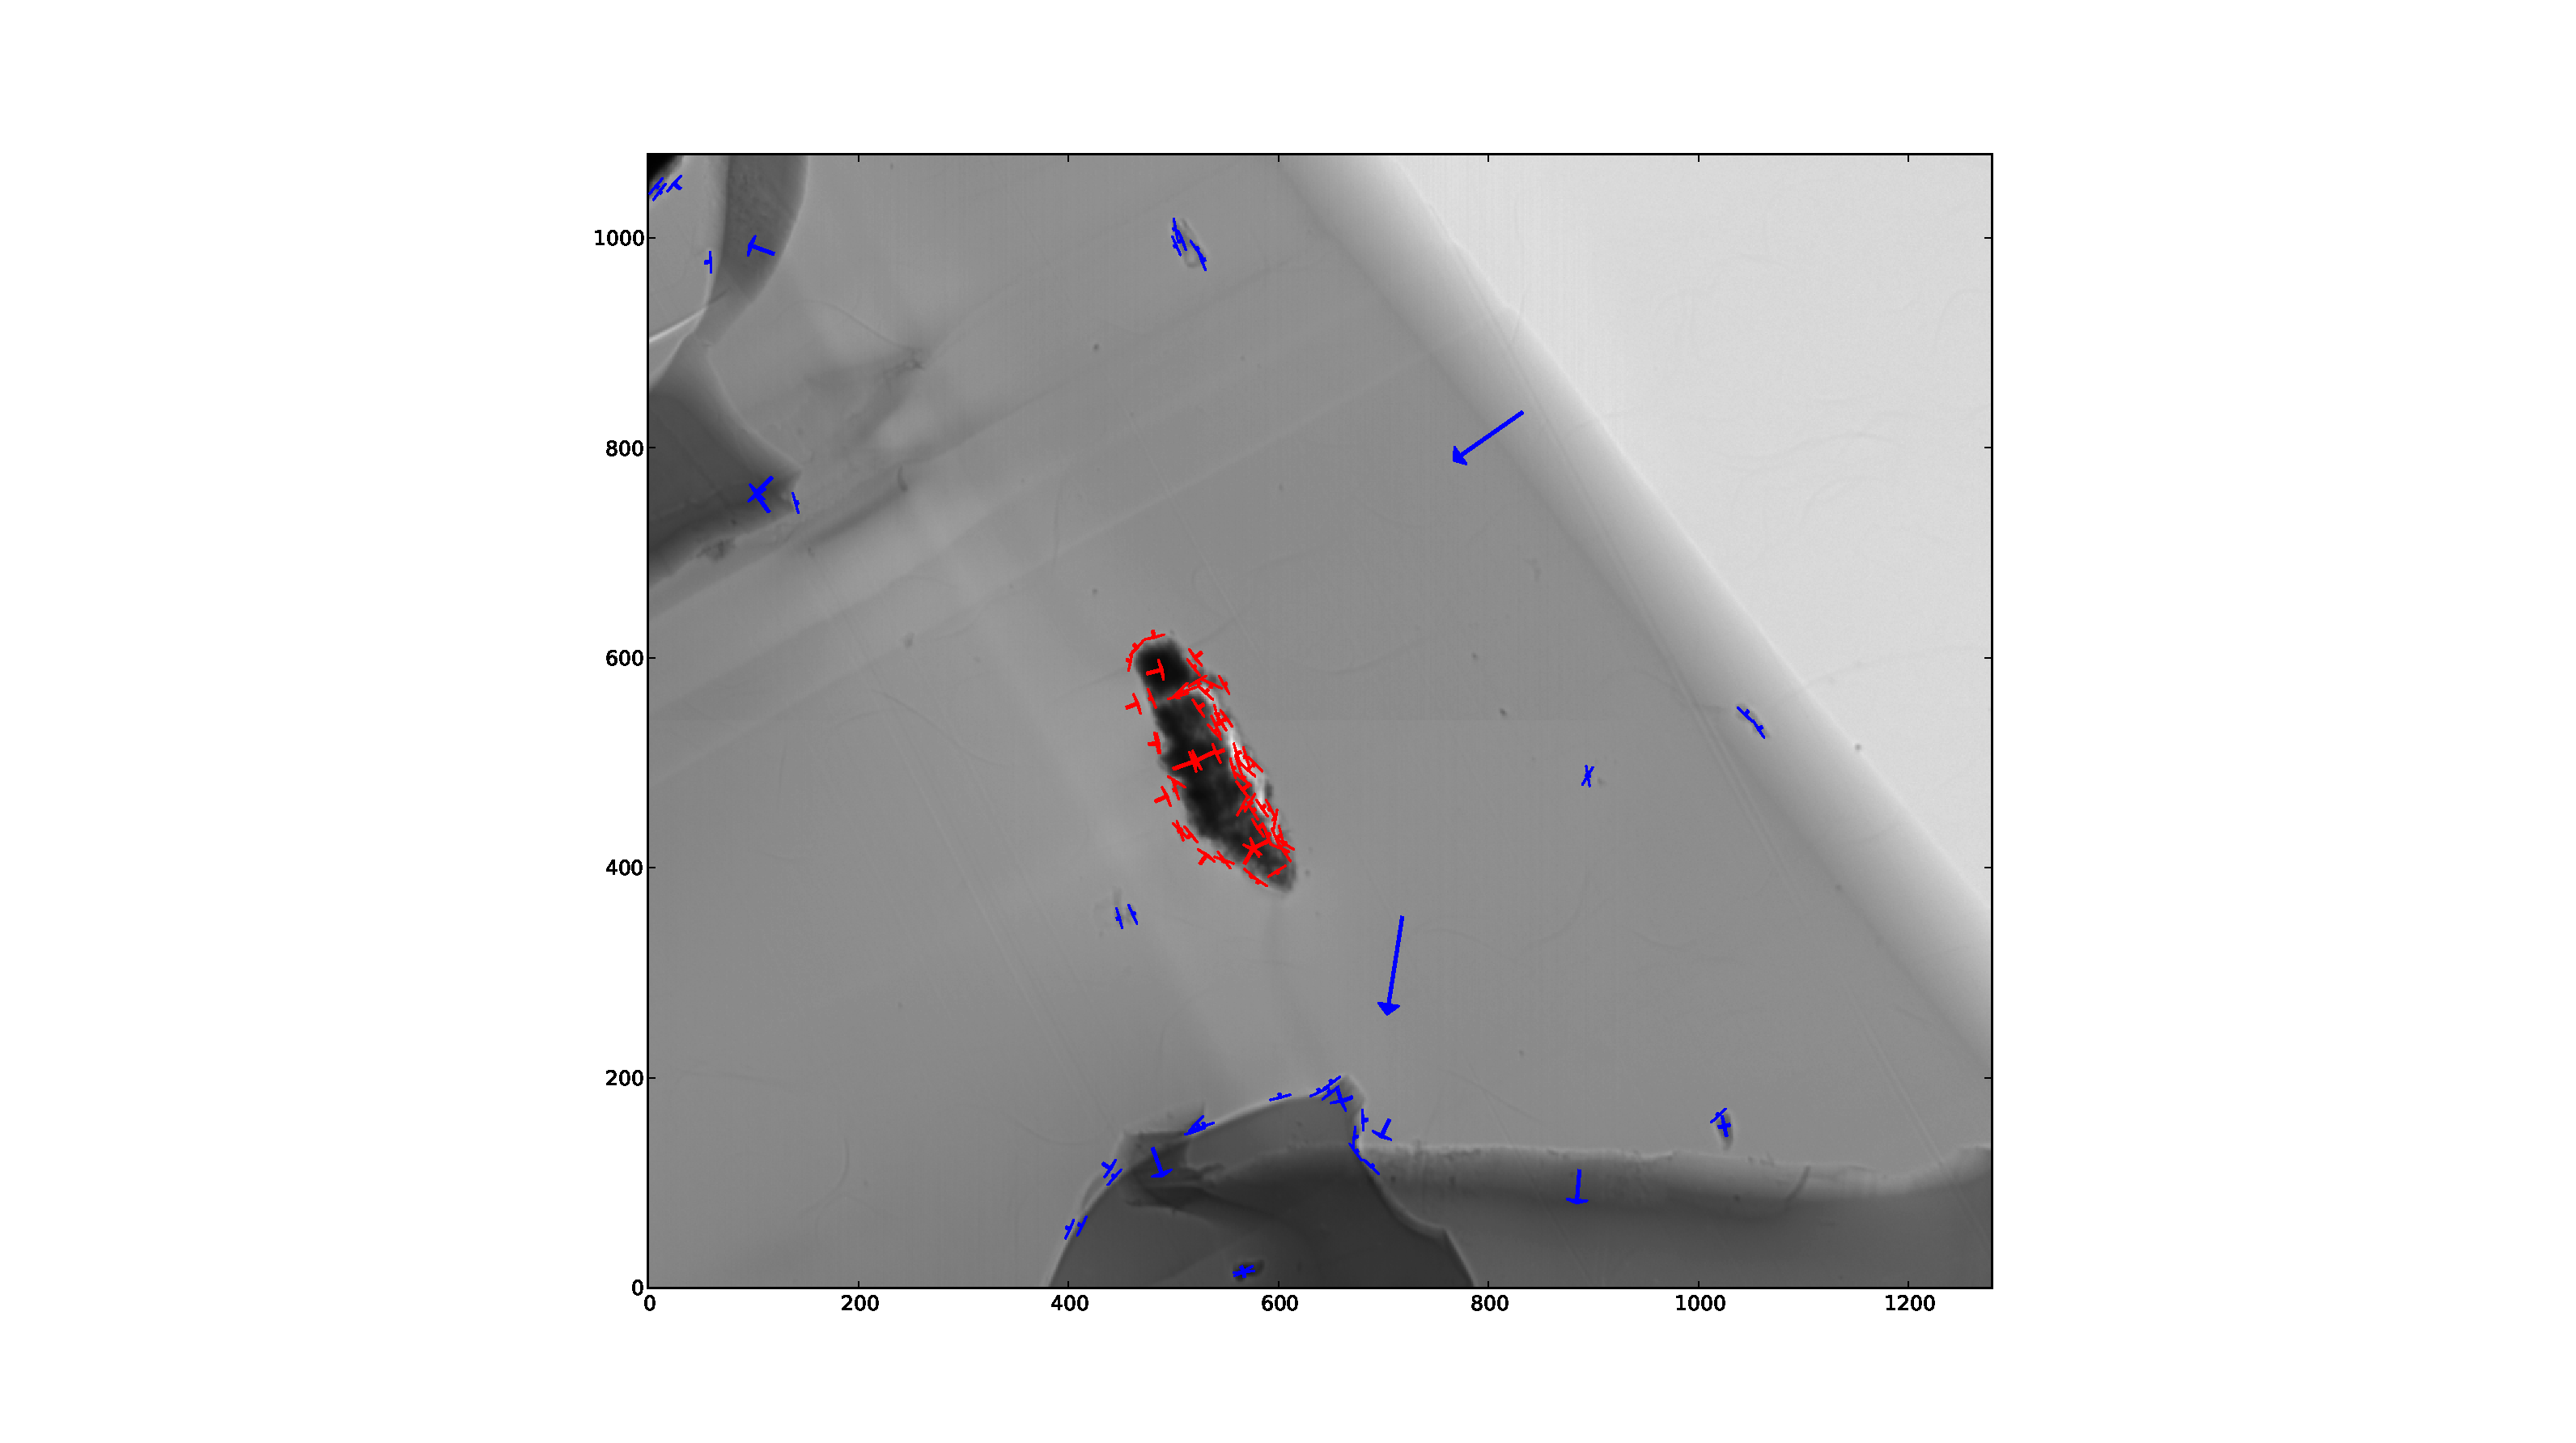
\includegraphics[width=15cm]{features.eps}
\caption{\label{sample} X-Ray radiograph of a thin section of painting
taken at ID21 at the suflur K-edge. Arrows represent the position of
SIFT-keypoints, in red those corresponding to the sample and in blue those from artifacts and from
the matrix.}
\end{center}
\end{figure}

The XANES stack alignment using phase correlation has failed in this sample,
probably due to the strong change in intensity on the borders (in this case 
between resin one the left side and air on the right side).

\subsection{SIFT algorithm overview}
% SIFT is an algorithm in computer vision which can be used for image alignment
% and pattern recognition.

%:\begin{itemize}
%%\setlength{\itemsep}{1pt}\setlength{\parskip}{0pt}\setlength{\parsep}{0pt}
%\item Keypoints detection: local extrema are detected in the \textit{scale-space} $(x, y, s)$. Every pixel is compared to its neighborhood in the image itself, and in the previous/next scale factor images.
%\item Keypoints refinement: keypoints located on corners are discarded. Additionally, a second-order interpolation is done to improve the keypoints accuracy, modifying the coordinates $(x, y, s)$.
%\item Orientation assignment: a characteristic orientation is assigned to the keypoints $(x,y,s, \theta)$
%\item Descriptor computation: a histogram of orientations is built around every keypoint, then concatenated in a 128-values vector. This vector is called \textit{SIFT descriptor}, it is robust to rotation, illumination, translation and scaling.
%\end{itemize}


The keypoints are detected in several steps according to Lowe's
original paper \cite{Lowe99}.
The scale variation is simulated by blurring the image:
a very blurred image represents a scene seen from a longer distance, where
small-scale details are not visible. Feature vanishing at a given scale are
local maxima when subtracting the next blurred from current image. Finally the
keypoint orientation and descriptor are obtained from gradient orientation
histograms.


\subsubsection{Keypoints detection:}

The image is increasingly blurred, by convolution with gaussian kernels, to
imitate the scale variations.
Then, consecutive blurs are subtracted to obtain the so-called differences of
gaussians (DoG) images where pixels are defined in a 3 dimensional
scale-space, composed by  their \emph{spacial} positions $(x, y)$ and their
\emph{scale} positions $s$ (related to the blur factor). Keypoints are
local maxima in this scale-space $(x, y, s)$.
%The point :$(x,y,s)$ is a local maximum  if\begin{itemize}
%\setlength{\itemsep}{1pt}
%\setlength{\parskip}{0pt}
%\setlength{\parsep}{0pt}
%\item $D(x-1, y, s) < D(x,y,s)$ and $D(x,y,s) > D(x+1, y, s)$ (local maximum in $x$)
%\item $D(x, y-1, s) < D(x,y,s)$ and $D(x,y,s) > D(x, y+1, s)$ (local maximum in $y$)
%\item $D(x, y, s -1) < D(x,y,s)$ and $D(x,y,s) > D(x, y, s+1)$ (local maximum in $s$)
%\end{itemize}
%\pic{0.7}{img/dog1.png}{Detection in scale-space (source: en.wikipedia.org)}



\subsubsection{Keypoints refinement:}

At this stage, many keypoints are not reliable: low-contrast keypoints are
discarded, and keypoints located on an edge are rejected in favour to those
staying on corners.
%For keypoints located on an edge, principal curvature across the edge is much
%larger than the principal curvature along it.
%The eigenvalues ratio $r$ of the Hessian matrix of the current DoG is compared
%to a threshold $\frac{(r+1)^2}{r} < R$.
To improve the keypoints accuracy, the coordinates are interpolated with a
second-order Taylor development.
%\[
% D \left( \vec{x} + \vec{\delta_x} \right) \simeq D + \frac{\partial D}{\partial \vec{x}} \cdot \vec{\delta_x} + \frac{1}{2} \left( \vec{\delta_x} \right)^T \cdot \left( H \right) \cdot \vec{\delta_x} \qquad \text{with } H = \frac{\partial^2 D}{\partial \vec{x}^2}
%\]
% Keypoints that were too far from a true (interpolated) extremum are rejected.


\subsubsection{Orientation assignment:}
In order to make SIFT descriptor invariant to rotation, they are calculated
relatively to the keypoint orientation; which is obtained using the following
procedure.
% The orientation
% of each keypoint is calculated so that SIFT descriptors can be invariant to rotation.
For each blurred version of the image, the gradient magnitude and orientation
are computed.
From the neighborhood of a keypoint, a histogram of orientations is built (36
bins, 1 bin per 10 degrees).
%\pic{0.7}{img/orientation.png}{Orientation assignment}
The maximum value of this histogram is the dominant orientation; it is defined
as the characteristic orientation of the keypoint.
Additionally, every peak greater than 80\% of the maximum generates a new
keypoint with a different orientation.



\subsubsection{Descriptor computation:}
Histograms of gradient orientations are built around every keypoint to define
its descriptor.
The neighborhood of a keypoint is divided into 4 regions of 4 sub-regions of 4x4
pixels.
In every sub-region, a 8-bin histogram is computed, then, all histograms
are concatenated in a 128-values descriptor.
The histogram is weighted by the gradient magnitudes and the current scale
factor in order for the descriptor to be robust with respect to rotation,
illumination, translation and scaling.


\section{Implementation}

While the phase correlation algorithm has been easily ported on graphics card
thanks to PyCUDA \cite{pyopencl} and cuFFT, and hence it is very fast and well
suited for online data pre-processing;
the SIFT implementation used at ESRF beamline ID21, based on \cite{ASIFT},
takes about 8 seconds per 4 mega-pixel frame  (a stack can contain up to  500
frames) using a single core.
Although the process is distributed using the EDNA framework \cite{edna} on a
16-core computer, the performance limits are constraining.

The SIFT algorithm, which is much more complicated than the phase
correlation algorithm, needed to be parallelized to benefit as well from modern
largely parallel hardware like graphics cards (GPU) to achieve the required
data rate.

SIFT\_PyOCL is a Python library implementing this algorithm for GPU
and other massively parallel compute devices.
% With the advent of high-performance GPU computing, several scientific data
% analysis programs for synchrotron radiation applications have already
% implemented effective parallelization schemes \cite{pynx,pyfai,pyhst2}
Like other synchrotron-centric tools \cite{pyhst2,pynx,pyfai} it benefited
from both a large scientific ecosystem built on NumPy \cite{numpy} and from
the high-performance computing capabilities of graphics cards.
%Image alignment being a crucial step in data pre-processing, we parallelized
% the SIFT algorithm to benefit from modern largely parallel
%hardware like graphics cards (GPU) to achieve a faster data rate.





\subsection{Parallelization of the algorithm}
Beside the \emph{Pythonic} interface, most of the
SIFT\_PyOCL code is divided in dozens of functions designed to be
executed in parallel and called kernels. Those kernels are written in Open
Computing Language (OpenCL) \cite{opencl} and  can be run on various
devices like GPU, multi-core CPU and accelerators.
They are launched subsequently from a Python module using PyOpenCL
\cite{pyopencl}, which provides both execution speed and code readability.
%The SIFT algorithm is used to align images with descriptors.
Once the above mentioned descriptors of two images are computed and matched, a
least-squares method is used to determine the transformation which will convert
keypoint positions of one image onto the keypoint positions of the other. For
now only affine transformations between images have been implemented in OpenCL
using bi-linear interpolation.
%All the steps, from descriptor computation to images alignment, are done on the device to benefit from its parallelism.

Unlike existing parallel versions of SIFT \cite{lu,rister,vasilyev}, the entire
process is done on the device to avoid time-consuming transfers between
central memory and device's memory.
This leads to several subtle tasks like the use of \emph{atomic} instructions,
or writing different versions of the same kernel to adapt it to various
platforms (CPU or GPU) and devices (e.g. \emph{compute capabilities} for
Nvidia GPUs).

The implementation of the first steps of the algorithm (keypoints detection and
refinement) did not raise any particular difficulty, since device parallelism
allows handling every pixel by a single thread.
Besides, convolution was implemented in the direct space (without Fourier
transform), currently up to 100 times faster than the convolution done in
the C++ reference implementation of IPOL \cite{ASIFT}
(and even faster, depending on the CPU/GPU pair).
A pyramid is used to represent the image in scale space \cite{Lowe04}.

The parallel implementation of the last steps (orientation assignment and
descriptors computation) was more complex.
For a given kernel, the performances strongly depend on the image
complexity and on the device the code is executed on.
Consequently, different versions have been written for a given kernel, each
adapted to different platforms and
devices; the optimal version being selected by the
Python module based on the \emph{compute capabilities} of the selected device.


\subsection{Installation and usage}
SIFT\_PyOCL, as any Python module, can be installed from its sources,
available on github \cite{sift_pyocl}.
Whilst SIFT\_PyOCL is open source and licensed under a very
permissive BSD license, the SIFT algorithm itself is
patented by the University of Columbia \cite{SIFT_pat}.
Nevertheless this patent does not apply in Europe.

Beside Python (version 2.6 or 2.7) and NumPy, SIFT\_PyOCL needs
PyOpenCL.
It was tested on the OpenCL drivers from Nvidia on a
large variety of their GPUs (Tesla, Fermi and Kepler generations) and on
multi-core processors with drivers from Intel and AMD.
The full installation procedure is simply (including testing):
\begin{verbatim}
$ python setup.py build test install
\end{verbatim}
Every single OpenCL kernel has been tested versus the reference
implementation and can be run without installing the library by
executing $test/test\_all.py$.
%(nota: not all kernels can run on all devices
%due to computing capabilities restrictions).

\subsection{Examples}

In this section we have collected some basic examples of how
SIFT\_PyOCL can be employed; using IPython \cite{ipython} in
Pylab \cite{matplotlib} mode.

\subsubsection{Extract keypoints:}
\begin{verbatim}
In [1]: import fabio
In [2]: img1 = fabio.open('image1.edf').data
In [3]: import sift
In [4]: siftplan = sift.SiftPlan(template=img1, devicetype="GPU")
In [5]: kp1 = siftplan.keypoints(img1)
\end{verbatim}

After having imported the FabIO \cite{fabio} module in [1], a first
absorption image is read in [2]. The SIFT\_PyOCL library is loaded in [3] and the
GPU is initialized in [4] with all memory allocated on the device (depending on
the image size).
In [4], the keypoint extraction takes 60 ms for a
4 mega-pixel image and returns a 261 keypoints vector as a numpy array named
\emph{kp1} (depending on the image).
%This figure varies a lot from sample to sample.

\subsubsection{Match keypoints between images:}
\begin{verbatim}
In [6]: img2 = fabio.open('image2.edf').data
In [7]: kp2 = siftplan.keypoints(img2)
In [8]: matchplan = sift.MatchPlan(devicetype="GPU")
In [9]: m = matchplan.match(kp1,kp2)
\end{verbatim}
A second image is read [6] and its keypoints are extracted [7].
In [8], a matching object is created, targeted to run on a graphic card.
Keypoint association is done in [9], returning a numpy array of 66 lines and 2
columns of matched keypoints (execution time: 2.7 ms), each keypoint having
attributes $x$, $y$, $scale$ and $angle$ in addition to the 128-byte descriptor.

\subsubsection{Align an image on a reference}
\begin{verbatim}
In [10]: aligner = sift.LinearAlign(img1,devicetype='GPU')
In [11]: img2_cor = aligner.align(img2)
\end{verbatim}
It is also possible to align directly an image on a reference frame using an
affine transformation: combination of translation, rotation, homothety,
reflection, etc.
An \emph{aligner} object is defined in [10] by instantiating the
\emph{LinearAlign} class from a reference image and the device type.
This \emph{aligner} contains keypoints of the
reference, a \emph{SiftPlan} and a \emph{MatchPlan} object plus the least square
refinement and bi-linear interpolation kernel.
The \emph{align} method performs keypoint extraction, matching, least-square
optimization of the affine transformation coefficients and finally applies the
correction to the frame [11], returning the corrected frame (execution time:
75 ms, all timing were measured on a Nvidia GeForce Titan GPU).

\subsection{Performances}

The SIFT\_PyOCL implementation has been compared with the SIFT
implementation from \cite{ASIFT} found on the IPOL server (reference
implementation) on a dual Intel E5-2667 (12 cores, 2.90GHz) with an Nvidia Tesla
K20m computer, Execution speed are summarized in Table \ref{bench}.
The acceleration measured on large images (more than 10 mega-pixels) is between
30 times and 100 times depending on the image complexity on the GPU, and from 4
times to 10 times when running on multicore-CPU.
Largest speed-ups have been obtained on large images thanks to the
great acceleration of Gaussian blurring.

\begin{table}
\caption{Execution time for typical FFXAS images (2560x2160) using different
implementations on a dual Intel E5-2667 (12 cores, 2.90GHz) with an Nvidia Tesla
K20m.}
\label{bench}
\vspace{1mm}
\begin{center}
\begin{tabular}{l l ccc}
Implementation & Driver & Keypoint extraction & Keypoint matching &
Image alignment\\
\hline
ASIFT        &   C++     &   3610 ms  & 95 ms  & --  \\
SIFT\_PyOCL  &   AMD  &   522 ms  &  21 ms&  578 ms \\
SIFT\_PyOCL  &   Intel  &   741 ms  &  13 ms&  843 ms\\
SIFT\_PyOCL  &   Nvidia  &    75 ms  &  5.8 ms & 90 ms\\
\end{tabular}
\end{center}
\end{table}



\subsection{Limitations}
While all calculations are performed in single precision floating point,
which is
compatible even with the oldest graphic cards supported by OpenCL, the
memory consumption has been traded off for performance.
Moreover, the algorithm is essentially suited
to linear colour scales; and  not suitable to high dynamic range
images like diffraction patterns.
% Neverthless, using the difference of gaussian method like in
% SIFT could be interesting for the extraction of spots for diffraction
% images.


\section{Future and prospects}


Registration of 3-dimensional objects would have a huge application potential,
especially in the field of tomography and medical images.
This field of research is very active in the frame of applied mathematics and
computer vision.


\section{Conclusion}

The SIFT algorithm is currently used at the ESRF ID21 beamline for full field
X-Ray absorption spectroscopy image alignment owing to its robustness against
scale, rotation and illumination changes.
The SIFT\_PyOCL Python module implements a parallel version of the SIFT
algorithm running both on graphic cards and on multi-core processors, with
interesting speed-ups.
Its programming interface tried to be simple to use and \emph{pythonic} while
supporting high performance computing ``under the hood''.
We believe it can be adopted by other software developers as general purpose
image alignment method; this is why the code was made open-source and free for
re-distribution.


\ack{Acknowledgements}

The author would like to thank the ID21 team, especially the beamline
responsible, Marine Cotte, Muriel Salomé and Barbara Fayard, who are in charge
of developing the full field XAS technique.
In the instrumentation division (ISDD) we would like to thank Claudio Ferrero,
head of data analysis unit, and Andy G\"otz, head of software group, for
supporting the parallelization work on this algorithm.
The Barnes foundation is also acknowledged for providing the painting fragment
which was used as example in this article and was originally studied to
understand the degradation of cadmium based pigments.
\bibliographystyle{iucr}
\bibliography{biblio}
%\referencelist[biblio]


\end{document}




